%%%%%%%%%%%%%%%%%%%%%%%%%%%%%%%%%%%%%%%%%%%%%%%%%%%%%%%%%%%%%%%%%%%%%%%%%%%%%%%%
\chapter{РАЗРАБОТКА МОДУЛЯ SIP-ТЕЛЕФОНИИ}
%%%%%%%%%%%%%%%%%%%%%%%%%%%%%%%%%%%%%%%%%%%%%%%%%%%%%%%%%%%%%%%%%%%%%%%%%%%%%%%%

В данном разделе описывается конфигурация окружения разработчика: сервер VoIP-телефонии b web-приложение. Приводится описание разработанных компонентов модуля SIP-телефонии для web-браузера.

\section{Конфигурация окружения разработчика}
\label{section:config}

В качестве web-приложения, в которое в дальнейшем будет встроен разрабатываемый модуль SIP-телефонии выберем SalesPlatform vtiger CRM. У данной CRM-системы исходный код находится в открытом доступе. В качестве сервера VoIP-телефонии был выбран сервер Asterisk, потому что vtiger CRM использует именно его для организации звонков сторонними (не браузерными) приложениями.

Однако работа модуля SIP-телефонии не зависит от того какой сервер соединяет клиентов в сети. Для связи клиентов можно было выбрать любой из серверов который поддерживает WebRTC. Список серверов был приведён в разделе \ref{subsection:reviewWebRTC}.

На сервер была установлена операционная система Debian GNU/Linux 8.4 (jessie). На эту машину был установлен сервер VoIP-телефонии Asterisk. На ней же установлена vtiger CRM.

\subsection{Настройка сервера VoIP-телефонии Asterisk}

По началу был установлен Asterisk 11 - первая версия сервера, поддерживающая WebRTC.\cite{asterisk} При его установке для работы WebRTC необходимо выбрать драйверы chan\_pjsip и chan\_sip и модули res\_srtp, res\_crypto и res\_http\_websocket. Затем был установлен FreePBX 12. FreePBX - это доступная через web-интерфейс графическая оболочка конфигурационных файлов Asterisk.\cite{FreePBX}

Через графический интерфейс FreePBX были созданы пользователи, им были присвоены номера, и включена возможность звонить с помощью WebRTC. Однако таким способом настроить работу сервера для работы с WebRTC не удалось. В качестве тестирования работы WebRTC была использована demo-версия браузерного SIP-телефона библиотеки sipML5.

Затем было предположенно, что для работы WebRTC, необходимо установить Asterisk последней версии 13.7.2. Так же был установлен FreePBX 13. Но с такой связкой тоже не удалось осуществить звонок с помощью WebRTC.

Тогда было решено не устанавливать FreePBX, и настроить Asterisk вручную, меняя конфигурационные файлы по инструкции в документации.\cite{asterisk} После такой настройки удалось осуществить звонок с помощью WebRTC.

В итоге на сервере установлен сервер IP-телефонии Asterisk 13.7.2. В конфигурационных файлах настроены звонки с номерами формата XXX, и добавлены внутренние номера, позволяющие звонить при помощи web-сокетов по порту 8088. Для этого создан DTLS-сертификат, и включена поддержка icesupport. Также добавлены номера, позволяющие звонить при помощи обычных сокетов по порту 5060.

При такой конфигурации сервера звонки могут осуществлятя между:
\begin{itemize}
\item двумя клиентами, использующими WebSockets
\item одним клиентом, использующим WebSockets и другим клиентом, использующим обычные сокеты
\item двумя клиентами, использующими обычные сокеты
\end{itemize}


\subsection{Настройка vtiger CRM}

Используемой CRM-системой является SalesPlatform vtiger CRM 6.4, которая работает на сервере Apache 2.4.10, в связке с PHP 5.6.22-0+deb8u1 и MySQL Server 5.5.49-0+deb8u1.

Файлы разрабатываемого модуля SIP-телефонии были помещены в корень CRM-системы. У vtiger CRM конечно имеется инструкция добавления новых модулей в систему, но не будем её использовать. Вместо этого сосредоточимся на разработке модуля SIP-телефонии, а не на том, как правильно его подключать.

\section{Разработка общих компонентов модуля SIP-телефонии}

Здесь рассмотрим разработку компонентов модуля, которые будут общими для любого web-приложения.

Итак, разрабатываемый модуль должен быть легко подключаем к web-приложению. Эта цель будет достигнута, если подключать разрабатываемый модуль одним файлом JavaScript. Поэтому было решено сделать файл softPhone.js, который подключает модуль softPhone.html AJAX-запросом. Файл SoftPhone.html включает в себя разметку кнопок плавающего окна, подключает аудио-файлы звонка и гудков, а также подключает остальные подмодули:
\begin{itemize}
\item SIPml-api.js - библиотека sipML5.
\item softPhoneCore.js - ядро модуля SIP-телефонии, отвечает за аутентификацию клиента на сервере SIP-телефонии, и осуществление звонков. Также в нём отслеживаются события звонка (CallEvents).
\item softPhonePopupUI.js - компонент обработки плавающего окна при перетаскивании мышью.
\item softPhone.css - разметка плавающего окна.
\item softPhone\_"web-app".js\footnote{здесь "web-app" означает название web-приложения, к которому будет подключатся модуль} - компонент, в котором размещается функция getSipAccount() для конкретного web-приложения.
\item softPhone\_"web-app".php - подмодуль, отправляющий sipAccountInfo клиенту.
\end{itemize}

Основные функции подмодуля softPhoneCore.js:
\begin{itemize}
\item createSipStack() - инициирует конфигурацию SIP-соединения, основываясь на информации полученной getSipAccount().
\item register() - аутентификация SIP-клиента на сервере.
\item unregister() - деаутентификация SIP-клиента на сервере, выполняется при закрытии web-страницы, если не было сделанно вручную.
\item onSipEventStack(e) - обработчик событий управляющей созданием или завершением SIP-сессий. Сессия аутентификации создаётся после аутентификации, а сессия звонка создаётся при входящем или исходящем звонке. Такие события поступают от сервера.
\item onSipEventSession(e) - обработчик событий SIP-сессий. Обрабатываются события ответа на звонок и сброса. Такие события поступают от собеседника.
\item call() - обработчик кнопки вызова.
\item hangup() - обработчик кнопки сброса.
\item finalState(action) - функция конечного автомата, управляющего состоянием SIP-клиента (см. рисунок \ref{image:FinalState}). В состоянии calling мы слышим гудки, а в состоянии incoming мы слышим рингтон. Также здесь происходит включение и выключение кнопок Call и HangUp.
\item startRingTone(), stopRingTone(), startRingbackTone() и stopRingbackTone() - функции воспроизведения и останова воспроизведения рингтона и гудков.
\end{itemize}

\begin{figure}[h!]
\center{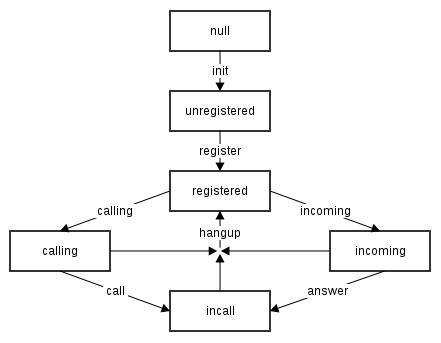
\includegraphics[width=0.75\linewidth]{FinalState}}
\caption{Конечный автомат, управляющий состоянием SIP-клиента}
\label{image:FinalState}
\end{figure}

Основные функции подмодуля softPhonePopupUI.js:
\begin{itemize}
\item show\_hide\_popup() - функция отображения и скрытия всплывающего окна.
\item mouseDown(e), mouseUp() и popupMove(e) - функции перетаскивания всплывающего окна.
\end{itemize}

\section{Встраивание модуля SIP-телефонии в CRM-систему}

Как уже было выбранно в разделе \ref{section:config} постараемся встроить наш модуль в web-приложение SalesPlatform vtiger CRM 6.4.

Чтобы подключить JavaScript файл к данной CRM-системе, необходимо в базе данных CRM-системы добавить в таблицу vtiger\_links запись c полями: linkurl - название файла (в нашем случае softPhone.js), linktype - HEADERSCRIPT, tabid - 0.\cite{vtiger_db} В этом случае скрипт будет выполнятся при каждой загрузке страницы.

Общие компоненты уже написаны. Теперь необходимо реализовать компоненты softPhone\_vtiger.js и softPhone\_vtiger.php зависимые от целевой CRM-системы.

Компонент softPhone\_vtiger.js реализует функции getSipAccount и callEvents, а компонент softPhone\_vtiger.php реализует функции sipAccountInfo и registerCallEvent (см. рис. \ref{image:architecture}).

Функция getSipAccount() осуществляет AJAX-запрос данных о SIP-аккаунте (ip-адрес и порт сервера телефонии, SIP-номер и пароль для текущего пользователя CRM-системы). А компонент softPhone\_vtiger.php отвечает на этот запрос. Для этого он анализирует данные о сессии пользователя, и, обращаясь к другим модулям CRM-системы, получает информацию о SIP-аккаунте текущего пользователя.

Так же компонент softPhone\_vtiger.js должен генерировать и отправлять данные о состоянии звонка, а softPhone\_vtiger.php должен их получать и генерировать карточки звонков, которые заполняются операторами.

Однако эти задачи трудоёмки для данной работы, так как исходный код данной CRM-системы очень большой, и поэтому выполнены не были. Получение информации о SIP-аккаунте было прописано только для одного пользователя. То есть любой пользователь, кто использует разработанный нами софт-фон, авторизуется за одного и того же пользователя на SIP-сервере. Так же не было реализовано создание карточек звонков в CRM-системе.

Для web-приложений, у которых есть API для получения информации о настройках SIP-аккаунта и API для получения информации о звонках, модуль softPhone\_vtiger.php будет отсутствовать. Эта информация будет получатся при помощи этих API из softPhone\_vtiger.js. Таким образом данный модуль не будет затрагивать изменения в серверной части web-приложения.

В данной CRM-системе за управление карточками звонка отвечает модуль PBXManager. В его функцию click-to-call было добавленно несколько строк кода, заполняющих поле набираемого номера в нашем модуле. То есть осуществив patch PBXManager, легко можно добавить click-to-call в разрабатываемый модуль.

\section{Резюме}

Рассмотрена конфигурация окружения разработчика. Рассмотрена разработка общих компонентов модуля SIP-телефонии для web-браузера. Так же рассмотренно встраивание модуля в web-приложение SalesPlatform vtiger CRM 6.4.
